\subsection{Space Density Evolution}
\label{Sec: Class Density}

\begin{figure*}
    \centering
    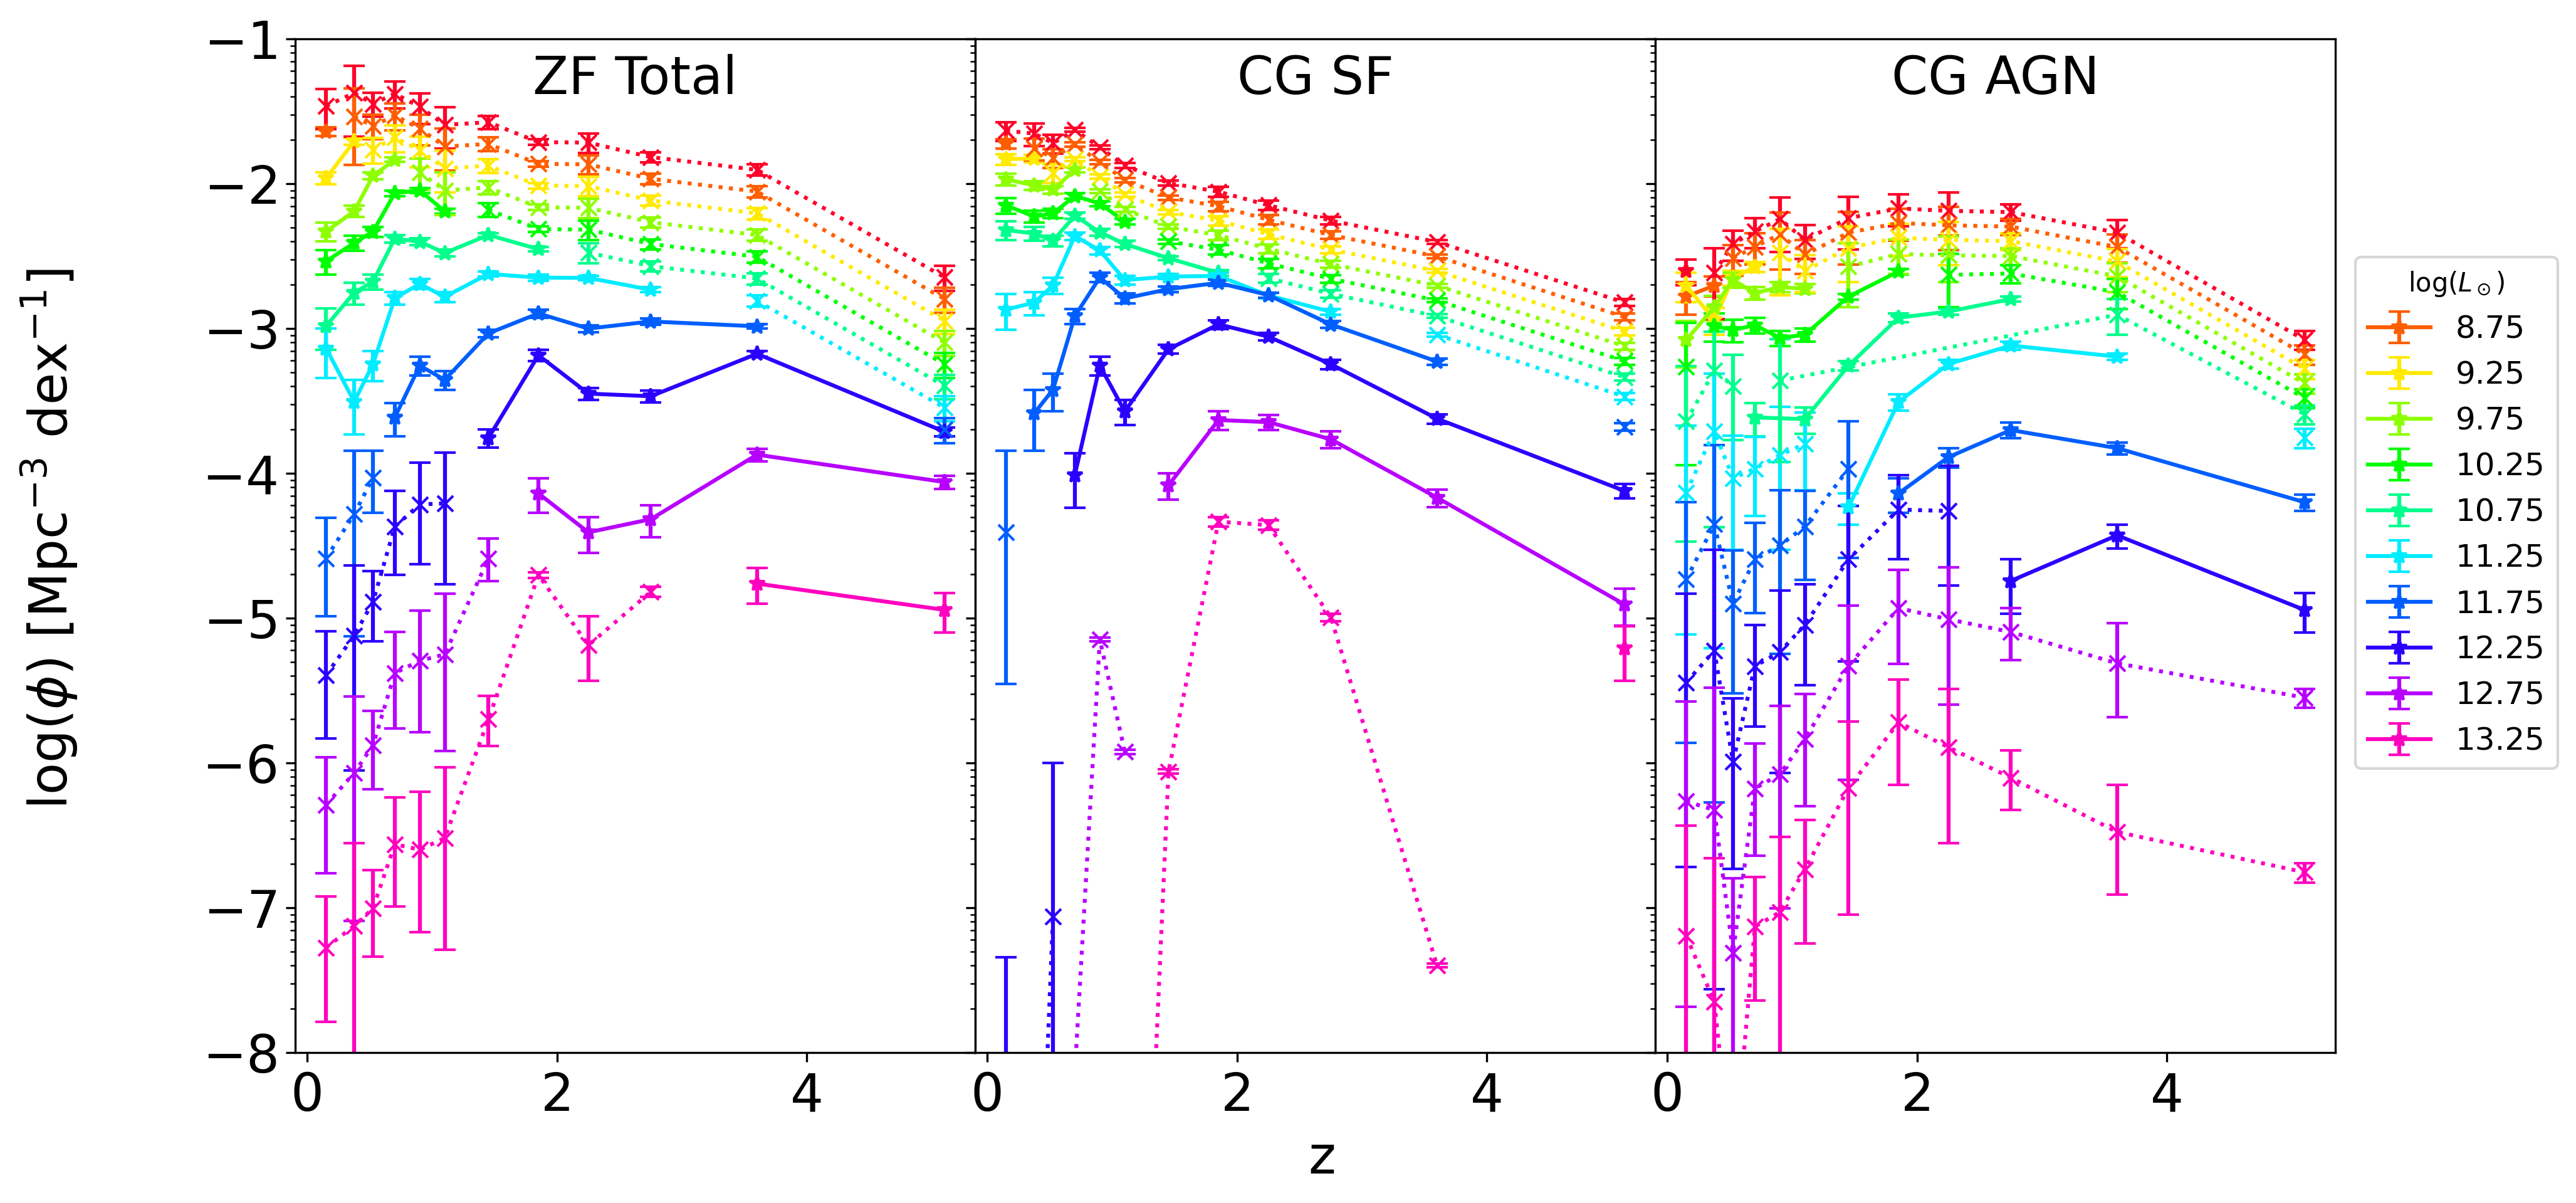
\includegraphics[width=\textwidth]{Figures/Class Evo.png}
    \caption{Luminosity class evolution as a function of redshift. $\phi$ values connected by straight lines correspond to real calculated values. $\phi$ values connected by dotted lines are estimated from the best fitting function (Schechter for CIGALE SF, Saunders for ZFOURGE Total and CIGALE AGN). Error bars represent the 1$\sigma$ uncertainty calculated with equation \ref{EQ: Vmax Error} for real values or derived from the function fitting process for estimated values. Real luminosity classes are 0.5 log$(L_{\odot})$ in width and centered in the middle (e.g 8.5 --- 9.0 is centred on 8.75). Estimated classes are calculated at the centre of the luminosity bin (e.g 8.75).}
    \label{Fig: Class Evo}
\end{figure*}

In this section, we inspect the evolution of different luminosity classes by visualising the number density of each luminosity bin across redshift (figure \ref{Fig: Class Evo}). By incorporating the class density evolution into our analysis, a better picture of the evolution of galaxies and the co-evolution of AGN can be ascertained. When possible, the $\phi$ values are taken from the existing luminosity bins\footnote{$\phi$ values were recomputed with luminosity bins $0.5\ \log_{10}(L_{\odot})$ wide}. Otherwise, $\phi$ values are calculated from the best-fitting LF. The class density evolution (figure \ref{Fig: Class Evo}) can be thought of as the transposition of the LF (figures \ref{Fig: Bolometric IR LF} and \ref{Fig: LF Filled}). The LF and class density are complimentary in that they allow us to view the number density both as an evolution with luminosity and redshift respectively. 

Figure \ref{Fig: Class Evo} results are significant. We present IR luminosity classes as low as $L_{IR}=10^{8.5} L_{\odot}$. We find that the space density of ZFOURGE LIRGs and ULIRGs have been consistently declining since at least $z=2$, and likely even earlier for ULIRGs. Galaxies fainter than LIRGs (FIRGs, $L_{IR} < 10^{11} L_{\odot}$) evolve very differently, beginning to decline at a lower redshift than their brighter luminosity counterparts. The redshift at which galaxies begin declining in number density is related to their luminosity. ZFOURGE galaxies fainter than $L_{IR} < 10^{9} L_{\odot}$ appear to be increasing in number density across all of cosmic time and have yet to begin declining. We find similar agreement in the literature with \cite{rodighiero_mid-_2010} and \cite{gruppioni_herschel_2013} with results mostly in agreement with ours. We attribute the differences to slight variations in the classes and methods within. We find that FIRGs dominate the ZFOURGE LD from $0<z<0.8$, declining from 74\% to 51\%. From $0.8<z<1.7$, LIRGs dominate LD, increasing slightly from 45\% to 47\%. At $z>1.7$, ULIRGs dominate LD, increasing rapidly from 59\% to 92\%. In the highest redshift bin, FIRG contribution drops to less 2\%

CIGALE SF galaxies evolve differently to ZFOURGE, although similar contributions to the LD are seen. FIRGs dominate LD density from $0<z<0.8$, declining from 80\% to 47\%. LIRGs only dominate LD from $0.8<z<1.2$ with 50\% contribution. ULIRGs dominate LD from $z>1.2$ onwards, generally increasing over time with some scatter. From figure \ref{Fig: Class Evo}, it is apparent that SF LIRGs evolve similarly to FIRGs at $z>2$. Although, the estimated $\phi$ values show increasing number density with decreasing luminosity for all FIRGs. One real $\phi$ value exists in the brightest luminosity class ($10^{13} < L_{IR} < 10^{13.5} L_{\odot}$) in our highest redshift bin which is only slightly lower in number density than the previous luminosity class. This is possibly evidence for the Saunders function being a good fit to the SF LF. A possible evolution scenario is theorised for SFG: all FIRGs evolve very similarly from high redshift to $z \approx 2$, increasing in number density from high redshift. At and below $z \approx 2$, the brightest FIRG number densities begin to peak and decline earlier than fainter FIRG counterparts which have yet to begin declining. LIRGs decline faster and earlier than FIRGs and ULIRGs decline faster and sooner than LIRGs. This reflects a \textit{downsizing} scenario in which brighter galaxies peak in number density at higher redshift \citep{merloni_synthesis_2008, wylezalek_galaxy_2014, fiore_agn_2017}.

CIGALE AGN again evolve very differently. Faint IR AGN dominate LD from $0 \leq z < 1.2$ and luminous IR AGN dominate LD from $z>1.2$ onwards. Ultra luminous IR AGN never dominate LD. Unlike SF galaxies, the difference between FIRGs and LIRGs is stark. There is a clear, systematic shift of the peak number density with luminosity class. The \textit{downsizing} seen in SF galaxies is more pronounced in AGN. As AGN luminosity increases, the number density of AGN peaks at higher redshifts and declines earlier than their fainter luminosity counter parts. When comparing the \textit{downsizing} effect between SFGs and AGN, it is unmistakable that galaxies with a luminous AGN decline faster and earlier than equally bright SFG counterparts.

% despite making up 98\% of sources at $z=0$, FIRGs only contribute 38\% of the total luminosity.

% LIRGs contribute only 2\% of the number density but make up 62\% of the total luminosity at $z=0$. At $z=2$, FIRGs contribute 46\% and 8\% of the total number density and luminosity respectively. LIRGS 45\% and 42\% respectively. ULIRGs, despite making up just under 10\% of the number density at $z=2$, contribute 50\% of the total infrared luminosity. FIRGs number and luminosity contribution drops to 0\% above $z=3$. In our final redshift bin, LIRG number and luminosity contribution is 21\% and 5\% respectively. ULIRG number and luminosity contribution is 79\% and 95\% respectively. However, these results only account for real measured galaxies and do not include the estimated galaxies. Otherwise, FIRGs would dominate the number density across all cosmic time.

% These results indicate that the brightest galaxies have been declining in number very shortly after the Big Bang. More luminous galaxies decline faster and at an earlier time period. Fainter galaxies take much longer to begin declining, if the faintest do at all.

% It is clear that ULIRGs decline much earlier than LIRGs, and LIRGs decline earlier than FIRGs. This presents a clear trend of brighter objects declining in number density more rapily than fainter galaxies.

% Across our data, we only have two luminosity bins between $10^{8.5} < L_{IR} < 10^{9}$ in the lowest redshift bin only, so results for this luminosity class could be improved in future work. Nevertheless, our results indicate very little number density evolution across all redshifts measured in our lowest luminosity class $L_{IR}=10^{8.5} L_{\odot}$. At $L_{IR}=10^{9} \& 10^{9.5} L_{\odot}$ there is again very little evolution until $z \approx 0.5$ when the number density again beings to decline. These results across a wider range of luminosities and redshifts previously measured in the literature confirm a \textit{downsizing} effect of all luminosity classes, of which the brightest galaxies begin declining before fainter ones.

% but only dominate the total luminosity in two redshift bins, $0.3 \leq z < 0.45$ and $0.6 \leq z < 0.8$. LIRGs dominate number density from $2 \leq z < 4$, but dominate luminosity from $0 \leq z < 0.3$, $1.0 \leq z < 1.7$, and $2.0 \leq z < 3.0$. From $0.45 \leq z < 0.6$, ULIRGs, despite only contributing 0.45\% to the number density, dominate the luminosity contribution with 42\%. ULIRGs only dominate the number density in our final redshift bin, and dominate luminosity from $1.7 \leq z < 2.0$, and $z>3$.

% \textcolor{red}{Our highest redshift bin (centered on $z=5.1$) is likely incomplete, and so the $\phi$ values here should be taken as a lower limit. In that case, it seems likely that LIRGs and ULIRGs have been declining in number density since at least $z=5$ when the universe was barely more than 1 Gyr old.}